% Tesis ITAM CLASS -- version 0.1 (13 - Abr - 2015)
% Clase para las tesis del ITAM
% 
% 13 - Abr - 2015 	Victor Martinez 	victor.martinez (at) itam.mx
% LICENSE: Creative Commons SA-BY 3.0
%
%
% Este documento presenta un ejemplo de uso de la plantilla
% El estudiante es libre de modificar este archivo a su gusto
% 
\documentclass{tesisITAM}
\usepackage[utf8]{inputenc}

\title{Implementación de un producto de datos}
\author{Miguel Angel Escalante Serrato}
\degree{Maestría en Ciencia de Datos}
\advisor{Adolfo de Unánue Tiscareño}
\year{2017}

\begin{document}

	\pagenumbering{gobble}
	\maketitle
	\publicationrights

	%%%%%%%%%%%%%%%%%%%%%%%%%%%%%%%%%%%%%%%%%%%%%%
	% ABSTRACT
	%%%%%%%%%%%%%%%%%%%%%%%%%%%%%%%%%%%%%%%%%%%%%%

	\begin{abstract}{spanish}
		Este documento presenta una plantilla para usar en las tesis y tesinas del ITAM. Se provee de manera gratuita y sin ninguna responsabilidad bajo la licencia \emph{creative commons BY-SA 3.0}.
	\end{abstract}

	\begin{abstract}{english}
		In this work we present a template for thesis and titulation works presented at ITAM. It is provided freely and without any responsability under the \emph{creative commons BY-SA 3.0}. 
	\end{abstract}


	\selectlanguage{spanish}
	\setcounter{page}{1}
	\pagenumbering{roman}

	\tableofcontents
	\listoffigures
	\listoftables
	\newpage

	\pagenumbering{arabic}
	\setcounter{page}{1}

	%%%%%%%%%%%%%%%%%%%%%%%%%%%%%%%%%%%%%%%%%%%%%%
	% CONTENT
	%%%%%%%%%%%%%%%%%%%%%%%%%%%%%%%%%%%%%%%%%%%%%%

	\chapter{Introducción}
\label{ch:intro}

\begin{chapterquote}{Leslie Lamport}
	Formal mathematics is nature's way of letting you know how sloppy
your mathematics is.
\end{chapterquote}

Este trabajo presenta una plantilla para las tesis y tesinas del Instituto Tecnológico Autónomo de México para los usuarios de \LaTeX \cite{lamport1994latex}. Nace de la necesidad de los matemáticos, actuarios e ingenieros (entre otras carreras) por utilizar un sistema de composición de textos adecuado para su trabajo de titulación. El objetivo es ayudar a la comunidad del ITAM a simplificar el proceso de escritura y edición de sus tesis, tesinas o casos. A continuación describimos a mayor detalle cada una de las partes de la plantilla.

\subsection{Descripción de los archivos}
\begin{enumerate}
\item El archivo \textbf{tesisITAM.cls} define una nueva clase de documento con el mismo nombre. Esta clase se basa en el tipo reporte, el cual se emplea comúnmente para reportes de trabajo, pequeños libros y tesis.

\item El archivo \textbf{macros.sty} define macros y operadores adicionales, como por ejemplo, el argumento mínimo $\argmin$. Además provee un espacio para que el estudiante agregue sus definiciones propias.

\item Este archivo \textbf{introduction.tex} describe el funcionamiento de la plantilla y de los archivos. 

\item El archivo principal \textbf{main.tex} es un ejemplo básico de un archivo de tesis para generar este ejemplo.

\item El archivo \textbf{portada.tex} contiene el código necesario para generar la portada. El archivo \textbf{derechos.tex} contiene el texto para cede de derechos de publicación hacia el ITAM.
\end{enumerate}

\subsection{Características de la plantilla}
La plantilla se basa en el documento tipo reporte. Todas las opciones de la clase \emph{report} pueden ser utilizadas sin ninguna modificación (a4paper, 10pt, etc...). El espaciado del texto se establece a 1.33. Se eliminó la identación del párrafo, y el espaciado entre párrafos fue disminuido. Las sub-secciones se numeran utilizando números romanos. Se define un encabezado para cada página (salvo las que inician un capítulo) donde aparece el número del capítulo y el nombre de la sección.

\subsubsection{Paquetes importados}
La plantilla utiliza los siguientes paquetes: \emph{graphicx}, \emph{amsopn}, \emph{fancyhdr}, y \emph{babel}. El paquete de manejo de idiomas babel es importado con los idiomas \textbf{english} y \emph{spanish} por defacto. Además, se seleccionan las opciones de uso de punto decimal y de nombrar las tablas como tablas y no como cuadros. 

\subsubsection{Opciones de clase}
Se declara una opción adicional de nombre \textbf{tesina} para cambiar la portada a que se declare el trabajo como tesina. 

\subsubsection{Campos para el autor}
Para el autor, se define los siguientes campos: \textbf{title},\textbf{author},\textbf{degree},\textbf{advisor}, y \textbf{year}. \emph{Title} define el título del trabajo de titulación, este título se presenta en la portada y al ceder los derechos de publicación. \emph{Author} define el nombre completo del autor de la tesis. \emph{Degree} se utiliza para establecer la carrera de la cual se va a titular, y debe incluir el texto completo (\emph{i.e.}, Licenciatura en X o Ingeniero en C). \emph{Advisor} recibe el nombre completo (con grado académico) del asesor, tal como se presentará en la portada. \emph{Year} recibe el año de titulación para presentarlo en la portada.

\subsubsection{Generando la portada}
El comando \textbf{\textbackslash maketitle} produce la portada con los campos previamente definidos. Utiliza el logo del ITAM, el cual se debe encontrar en el \textbf{PATH} de \LaTeX (\emph{e.g.}, en el fólder de Figures). 

\subsubsection{Cediendo derechos de publicación}
El comando \textbf{\textbackslash publicationrights} imprime una página con el texto oficial de cede de derechos. Los nombres de la tesis (tesina) y del autor se obtienen de los campos previamente definidos.

\subsubsection{Añadiendo el resumen}
Comúnmente, el resumen (o \emph{abstract}) se debe escribir tanto en español como en inglés. Para esto, se define el ambiente \textbf{abstract} que recibe como parámetro un idioma. En el caso de que el idioma no sea ni inglés ni español, se recomienda que el idioma haya sido previamente importado como opción del paquete babel. En otro caso, el paquete imprimirá una advertencia. 

\subsubsection{Citando a los grandes}
La plantilla define un nuevo ambiente para las citas al principio del capítulo \textbf{chapterquote} que recibe dos parámetros: el autor y el texto. Para un ejemplo, referirse al principio de este capítulo.


\section{Licencia}
Esta plantilla se distribuye bajo la licencia \emph{creative commons BY-SA 3.0}. Esta licencia permite la modificación de cualquier aspecto de la plantilla siempre y cuando se respeten las siguientes condiciones:
\begin{enumerate}
	\item Que se mantenga la atribución del trabajo original, es decir, que se mencionen los autores originales y su afiliación, tal como se hace en el archivo original.
	\item Que todas las modificaciones se hagan públicas y libres de acceso, sin recibir ningún tipo de retribución por el uso o distribución de la plantilla.
\end{enumerate}

\section{Autor}


	% \chapter{Revisión de Literatura}
\label{ch:relatedwork}

%This paper is related with empirical studies around two topics: measuring minimum wage's impact and 

\section{Salario mínimo}
%There exist wide variety of literature around the impact of increasing the minimum wage for developing countries. Estimates of the elasticity of employment with respect to minimum wage are generally small and heterogeneous (Neumark \& Munguia Corella, 2019). The evidence suggests that for the mexican context, especially when employers have monopsonic power, the impact of the minimum wage in employment can be small or insignificant. On the other hand, increasing the minimum wage can impact income and the percentage of work income that is reported to IMSS (Munguia Corella, 2020).

\noindent Existe una amplia literatura sobre el impacto del aumento al salario mínimo en países en vías de desarrollo. Estimaciones de la elasticidad del empleo respecto al salario mínimo son generalmente pequeñas y heterogéneas \citep{neumark_2019}. La evidencia entonces sugiere que para contextos como el mexicano, sobre todo en situaciones en que las empresas tienen poder monopsónico, el impacto del salario mínimo en el empleo puede ser muy pequeño o nulo. No obstante, el aumento del salario mínimo sí impacta los ingresos laborales y el porcentaje de los ingresos laborales que se reportan al IMSS \citep{munguia_2020}. 


%In respect to the Mexican case, the minimum wage increase in ZLFN with respect to the rest of the country in 2019 came with an important number of research papers that attempt to measure its impact on employment and salaries. On one hand, reports by Banco de México and some other researchers find a negative effect in employment \citep{banxico2020} and prices \citep{banxico2020, calderon2020}. On the other hand, other authors find no such impact in employment \citep{campos-vazquez_delgado_rodas_2020} nor in prices \citep{campos-vazquez_esquivel_2020}, but they recognize that it could be caused in part by VAT's decrease that came with the minimum wage increase.
 
 

Respecto al caso mexicano, el aumento del salario mínimo diferenciado en la ZLFN con respecto al resto del país en 2019 vino acompañado de un número importante de artículos de investigación que buscan medir su impacto en el empleo y los salarios. Por un lado, los estudios realizados por Banco de México y algunos otros investigadores señalan que sí hubo efectos negativos en la generación de empleo \citep{banxico2020} y en los precios \citep{banxico2020, calderon2020}. Sin embargo, otros autores no encuentran efectos significativos en el empleo \citep{campos-vazquez_delgado_rodas_2020} ni en los precios al consumidor \citep{campos-vazquez_esquivel_2020}, aunque reconocen que puede deberse en parte a que el aumento al salario mínimo en 2018 fue acompañado de una disminución del Impuesto al Valor Agregado (IVA). La propia Comisión Nacional de los Salarios Mínimos, en su reporte del 2019, concluye que el aumento salarial no provocó efectos negativos en la generación de empleo.

%With respect to mortgages, there exists evidence that exogenous shocks to credit supply can affect housing prices \citep{imbs_favara_2010}. Since house prices can affect a households' wealth, movements in the housing market can modify consumption decisions. Also, a property's values influence firms' and families' location decisions. In a macro setting, housing prices have played an important role in recent business cycles. Then, public policies aimed at increasing credit supply must take into account the aforementioned effects.

A pesar de estas diferencias, los artículos antes mencionados coinciden en que, para el caso de México, los efectos sobre el empleo parecen no ser significativos. Además, la mayoría de los estudios coinciden en que esta política sí tuvo como consecuencia un aumento en los salarios de cotización ante el IMSS. 


\section{Vivienda}

\noindent La construcción de desarrollos habitacionales de bajo costo fue un pilar fundamental de la política pública de países desarrollados durante el s. XX \citep{monkkonen_2011}. Sin embargo, a partir del s. XXI, el paradigma cambió hacia una política habitacional que dejó en manos del mercado inmobiliario la construcción de nuevos asentamientos. La política pública tomó un enfoque de oferta, otorgando subsidios o beneficios fiscales para que las empresas inmobiliarias construyeran viviendas de bajo costo. Sin embargo, estas viviendas se construían principalmente en la periferia de las ciudades, lejos del transporte público y otros servicios; ello provocaba  segregación y pérdidas en bienestar para la población de menores ingresos. La literatura indica que vivir en asentamientos lejos del centro económico de las ciudades en países en desarrollo puede impactar la experiencia laboral de los jóvenes \citep{franklin_2018,kain_1992} y la mayoría de los propietarios prefieren abandonarlos \citep{barnhardt_2017}. 

 
En contraste, soluciones por el lado de la demanda pueden mejorar la movilidad intergeneracional de las personas con menores ingresos. Por ejemplo, para el contexto de Estados Unidos, individuos que se mudaron a zonas de baja pobreza antes de cumplir trece años tienen, significativamente, mayor escolaridad e ingreso con respecto a sus congéneres que no se mudaron \citep{chetty_hendren_katz_2016,chetty_hendren_2018}. Adicionalmente para el contexto de familias estadounidenses viviendo en barrios urbanos marginados, existe evidencia de beneficios importantes derivados de mudarse fuera de zonas con altos niveles de pobreza, tales como menores tasas de obesidad, diabetes y, en general, menores afectaciones psicológicas y menor prevalencia de depresión y ansiedad \citep{kling_liebeman_katz_2007}. Por tanto, fomentar que trabajadores de bajos ingresos puedan acceder a vivienda en mejores vecindarios puede expandir sus posibilidades de desarrollo.


En cuanto al crédito hipotecario, existe evidencia de que shocks exógenos a la oferta de crédito pueden afectar los precios de las viviendas \citep{imbs_favara_2010}. Saber si movimientos en la oferta de crédito hipotecario afectan directamente a los precios del mercado inmobiliario es crucial para políticas públicas. El valor de las propiedades inmobiliarias afecta el ingreso de los hogares y por tanto puede impactar sus decisiones de consumo. Además, determina la ubicación de los hogares y de las firmas. En un nivel macro, los precios de los hogares han jugado un papel importante en los ciclos de negocios recientes.

%Since houses are usually used as collateral for mortgages, there is endogeneity between housing credit supply and housing prices. A way to explore the impact of credit booms is to exploit politically motivated policies that impact the credit supply but do not correlate with housing prices. In my case, I propose the minimum wage increase in ZLFN for such analysis.

En cuanto al crédito hipotecario, ya que regularmente el colateral es un propiedad es difícil aislar el efecto de los precios de vivienda en la oferta de hipotecas. Es decir, la relación entre el precio de las viviendas y el crédito hipotecario es endógena. Un camino para identificar el impacto de movimientos en la oferta crediticia en los precios de vivienda es explotar el impacto de decisiones políticas que mueven la oferta de crédito pero no los precios \citep{imbs_favara_2010}. En ese sentido, a mi me interesa explotar el aumento del salario mínimo en la ZLFN.

%Also, recently there is renewed interest around the progressivity of increasing the minimum wage. There is evidence that the channels by which increasing the minimum wage affects consumers are more diverse than was thought of. Apart from the traditional channels (e.g. unemployment, income, consumption), even retail prices can be negatively affected by increasing the minimum wage \citep{leung_2020}. There are arguments to think that spillover to the housing market might happen, which in turn makes housing rents go up \citep{macurdy_2015,yamagishi_2018,agarwal_ambrose_diop_2019}.
%Since low earners tend to rent rather than own a house, this might influence welfare negatively.

Además, en un contexto reciente donde se cuestiona que subir el salario mínimo sea una medida progresiva, hay razones para pensar en el mercado inmobiliario como un canal por el cual se diseminan los efectos del aumento al salario mínimo. Existe evidencia de sobra sobre el resultado de subir el salario mínimo en el ingreso, el consumo y el desempleo por citar ejemplos, e incluso sobre los precios minoristas \citep{leung_2020} . Recientemente se ha encontrado que las subidas de salario mínimo terminan causando que suban las rentas \citep{macurdy_2015,yamagishi_2018,agarwal_ambrose_diop_2019} y dado que quienes menos ganan tienden a rentar en vez de poseer vivienda, no podemos asegurar que su bienestar mejore.

	% \include{Chapters/method}

	% \chapter{Resultados}
\label{ch:results}

%\begin{chapterquote}{Leslie Lamport}
%	Formal mathematics is nature's way of letting you know how sloppy
%your mathematics is.
%\end{chapterquote}

\noindent Los coeficientes $\beta_t$ que resultan de estimar la ecuación \ref{eq:1}, así como sus intervalos de confianza al 95\% con errores estándar cluster , se muestran en la Gráfica \ref{fig:1}. Las Gráficas \ref{fig:2} y \ref{fig:3} muestran los resultados de la misma regresión, pero restringida a las submuestras de salarios bajos y altos respectivamente. Los coeficientes $\beta_t$ que resultan de estimar la ecuación \ref{eq:2}, así como sus intervalos de confianza al 95\% con errores estándar cluster, se muestran en la Gráfica \ref{fig:4}. Las Gráficas \ref{fig:5} y \ref{fig:6} muestran los resultados de la misma regresión, pero restringida a las submuestras de salarios bajos y altos respectivamente.

En la primera parte de mi análisis, observo que el efecto del incremento al salario mínimo en la ZLFN sobre el empleo fue pequeño o inexistente. Esto se ilustra en la Gráfica \ref{fig:1} de resultados, donde se aprecia que los coeficientes de diferencias en diferencias para todos los años son cercanos a cero. Además, este comportamiento se mantiene después del aumento del salario mínimo en la ZLFN. Casi todos los intervalos de confianza de los coeficientes \textit{diff-in-diff} contienen al cero, salvo el correspondiente al segundo trimestre de 2019. La inclusión del cero en el intervalo de confianza indica en que el impacto del aumento al salario mínimo en la ZLFN sobre el empleo no fue estadísticamente significativo.      

\begin{figure}[H]
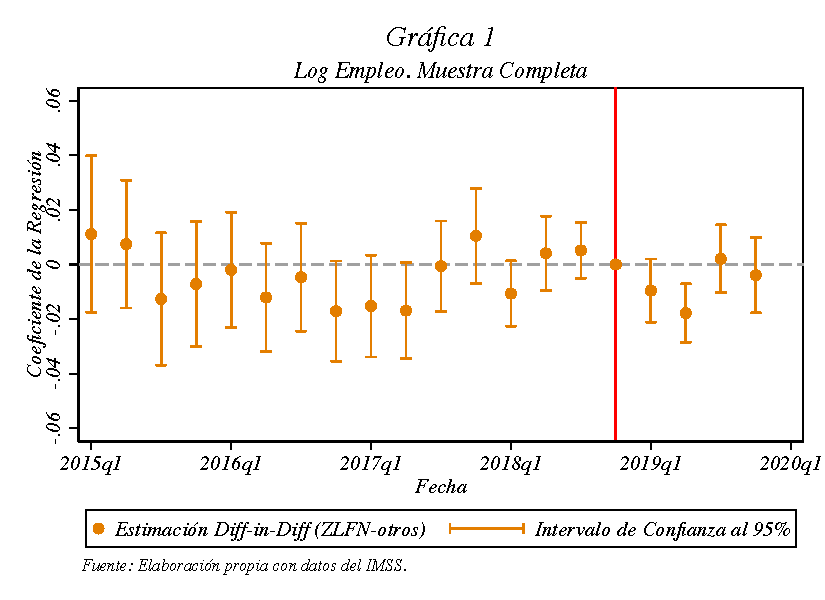
\includegraphics[width=0.9\textwidth]{Figures/LogEmpleo_MuestraCompleta.pdf}
\caption{Impacto del aumento en el salario en el empleo. Muestra completa.}
\label{fig:1}
\end{figure}


Es posible que la falta de un impacto significativo se deba a que el aumento al salario mínimo solamente afecta al empleo en la cola izquierda de la distribución de salarios, que contribuyen poco al empleo agregado. Sin embargo, al separar a los trabajadores por nivel salarial se aprecia que esto no es el caso. Si nos enfocamos únicamente en la submuestra de empleos bajos, es decir, gente que gana menos de dos salarios mínimos, vemos que todos los intervalos de confianza de los coeficientes \textit{diff-in-diff} contienen al cero. Efectivamente, si hacemos el mismo ejercicio para la submuestra de empleos altos, vemos que la anomalía vista en la muestra completa durante el segundo trimestre de 2019 se suscita por trabajadores pertenecientes a esta submuestra. Al observarla segunda gráfica se observa que, para la población de menores ingresos, un incremento al salario mínimo no tiene impactos sobre el empleo. Para la población en su totalidad, también es posible decir que el efecto del incremento al salario mínimo en la ZLFN es pequeño o nulo.

\begin{figure}[H]
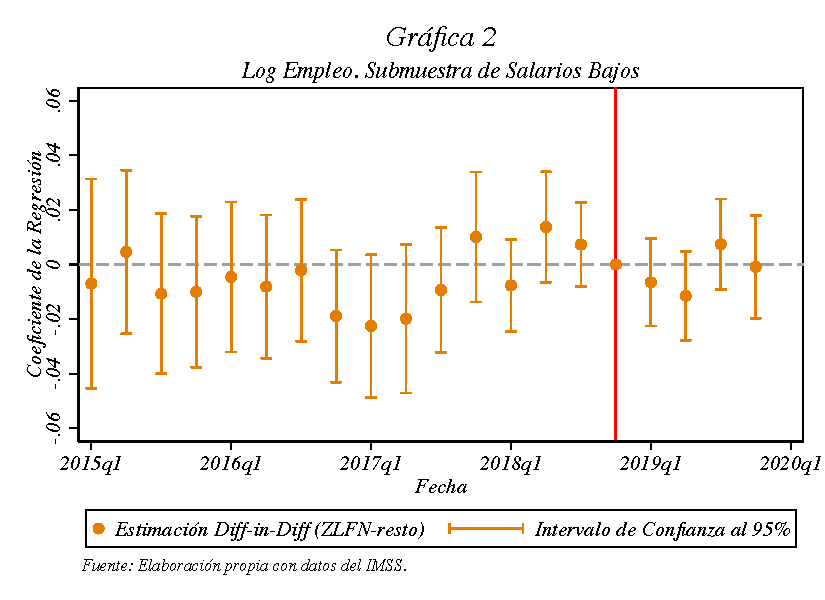
\includegraphics[width=\textwidth]{Figures/LogEmpleo_SalariosBajos.pdf}
\caption{Efecto del aumento del salario mínimo en el empleo. Submuestra salarios bajos.}
\label{fig:2}
\end{figure}

\begin{figure}[H]

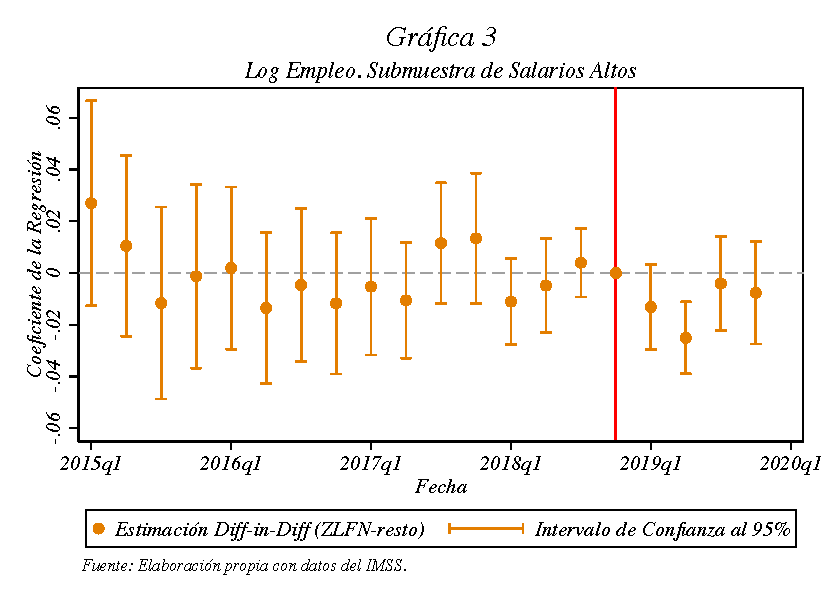
\includegraphics[width=\textwidth]{Figures/LogEmpleo_SalariosAltos.pdf}
\caption{Efecto del aumento del salario mínimo en el empleo. Submuestra salarios altos.}
\label{fig:3}
\end{figure}

Sin embargo, sí hay un impacto significativo sobre los salarios para todos los trabajadores, sobre todo dentro de la población de menores salarios. Al separar nuevamente a los trabajadores por nivel de salario, se observa que el aumento salarial causado por subir el salario mínimo es mucho mayor para niveles bajos de salarios que para niveles altos de salarios.

Los coeficientes que resultan de mi estrategia de diferencias en diferencias son estadísticamente significativos y positivos. Es decir, los salarios de cotización ante el IMSS de la ZLFN aumentan en mayor medida (aproximadamente 10\%) que el resto del país, producto del aumento diferenciado al salario mínimo en 2019. Además, al separar a los trabajadores por nivel salarial, encuentro que el efecto es mayor  para los trabajadores con menores salarios. Una explicación es que existe complementariedad entre ambos tipos de trabajos, otra que los salarios bajos se usan de referencia al negociar los salarios altos (el llamado efecto faro).

\begin{figure}[H]
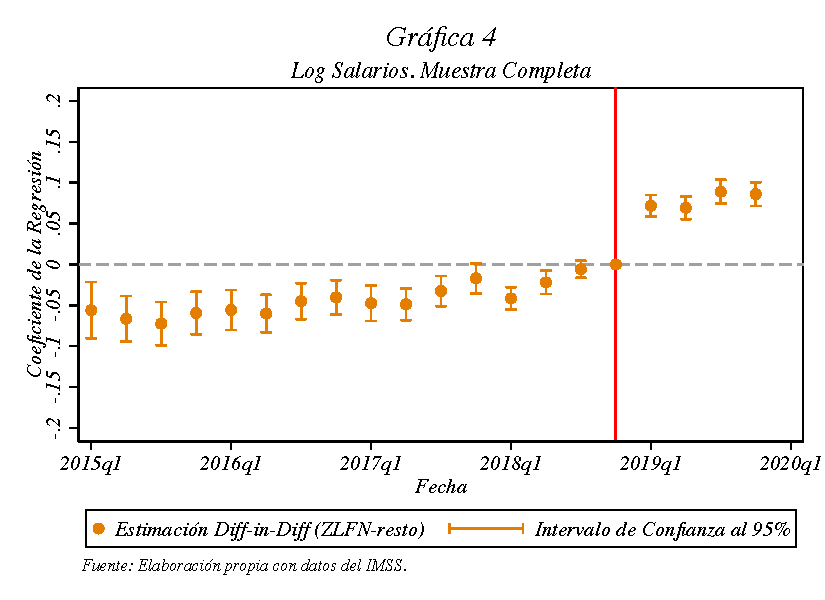
\includegraphics[width=\textwidth]{Figures/_LogSalarios_MuestraCompleta.pdf}
\caption{Efecto del aumento del salario mínimo en los salarios. Muestra completa.}
\label{fig:4}
\end{figure}

\begin{figure}[H]
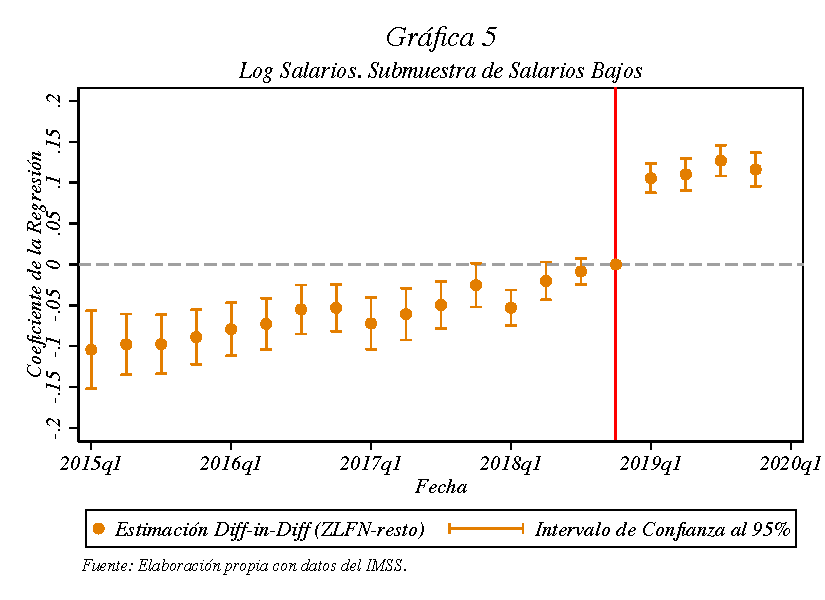
\includegraphics[width=\textwidth]{Figures/_LogSalarios_SalariosBajos.pdf}\caption{Efecto del aumento del salario mínimo en los salarios. Subuestra salarios bajos.}
\label{fig:5}
\end{figure}

\begin{figure}[H]
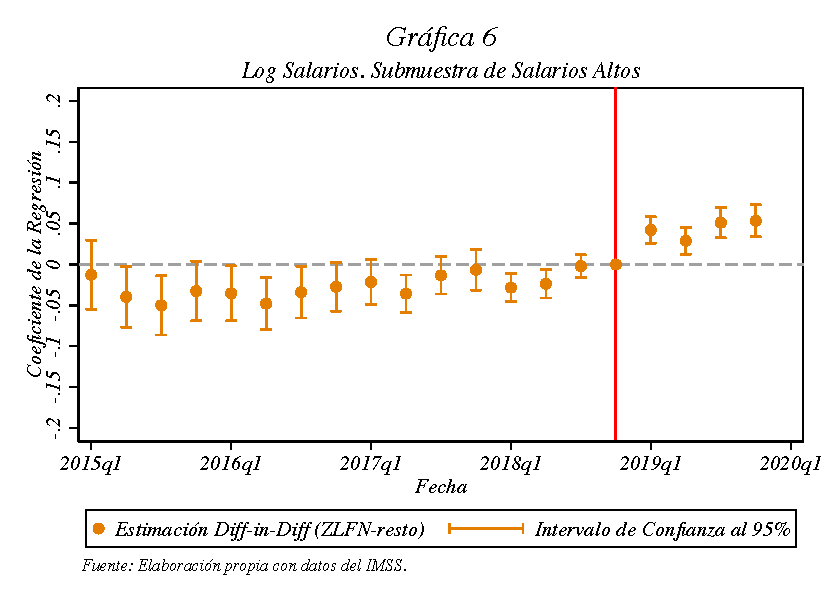
\includegraphics[width=\textwidth]{Figures/_LogSalarios_SalariosAltos.pdf}\caption{Efecto del aumento del salario mínimo en los salarios. Submuestra salarios altos.}
\label{fig:6}
\end{figure}

En resumidas cuentas, con respecto a la primera parte de mis estimaciones, subir el salario mínimo sí aumenta el salario de cotización de los trabajadores, sobre todo aquellos de bajos salarios, sin tener impacto significativo sobre el nivel de empleo. 

Si bien los coeficientes de la gráfica \ref{fig:4} antes de aumentar el salario mínimo muestran una suave tendencia creciente, el mayor cambio de un periodo a otro no excede 0.03. mientras,el cmabio después de aumentar el salario mínimo es de casi 0.1. Una historia similar puede contarse sobre las tendencias pre aumento del salario mínimo de \ref{fig:5} y \ref{fig:6}.

Para la segunda parte, resumo en tablas los coeficientes de las regresiones estimadas para ambas variables dependientes, cambiando solamente la medida de intensidad estatal. Los resultados de las regresiones \ref{eq:3} y \ref{eq:4} se muestran en las Tablas \ref{tab:2} y \ref{tab:3}, respectivamente.


Los datos expuestos en las Tablas \ref{tab:2} y \ref{tab:3} están redondeadas a tres cifras significativas. Observando la Tabla \ref{tab:2} se observa que, sin importar la medida que se opte por usar, el efecto de subir el salario mínimo es positivo , pero no estadísticamente significativo sobre el número de créditos. Es posible apreciar que, para la hipótesis nula de que los coeficientes son cero, el p-value para $\beta$ es alto sin importar cuál medida de intensidad estatal se utilice, por lo cual los coeficientes no son estadísticamente significativos. 

Aquí he estimado el coeficiente  que pondera al tratamiento, es decir el periodo a partir del cual se hace el aumento al salario mínimoy a la medida de intensidad estatal. Recordemos que esta medida es un proxy de qué tanto se ve afectada cada entidad federativa por la medida. Los resultados de las regresiones indican que el aumento al salario mínimo no trajo consigo un efecto significativo sobre el número de créditos otorgado por el INFONAVIT a trabajadores. Este primer resultado no es sorprendente, dado que el acceso a créditos INFONAVIT depende principalmente de contar con un salario formal y el aumento al salario mínimo no parece haber impactado de forma importante al total de empleos.

\begin{table}[H]
\caption{Impacto del aumento al salario mínimo en la ZLFN sobre el número de créditos INFONAVIT otorgados}
\label{tab:2}
\begin{adjustbox}{max width=\textwidth}
\begin{tabular}{lcccc}

\hline \\
 & & Logaritmo & de créditos & INFONAVIT  \\
 &  &  &  &  \\
Medidas de intensidad estatal & (1) & (2) & (3) & (4)  \\ \hline
 &  &  &  &  \\
\% de trabajadores que ganan entre 1 y 2 salarios mínimos que viven en la ZLFN & 0.00656 &  &  &  \\
 & (0.0852) &  &  &  \\
\% del total de empleos de trabajadores que ganan entre 1 y 2 salarios mínimos que viven en la ZLFN &  & 0.00902 &  &  \\
 &  & (0.285) &  &  \\
\% de trabajadores que ganan menos de 2 salarios mínimos que viven en la ZLFN &  &  & 0.00915 &  \\
 &  &  & (0.286) &  \\
\% del total de empleos de trabajadores que ganan menos de 2 salarios mínimos que viven en la ZLFN  &  &  &  & 0.00660 \\
 &  &  &  & (0.0852) \\
Constante & 7.959*** & 7.960*** & 7.960*** & 7.959*** \\
 & (0.0315) & (0.0315) & (0.0315) & (0.0315) \\
 &  &  &  &  \\
 Effectos fijos por estado  &  Sí &  Sí &  Sí & Sí \\
  Effectos fijos por periodo  &  Sí &  Sí &  Sí & Sí \\
Observaciones & 496 & 496 & 496 & 496 \\
 R-cuadrada & 0.975 & 0.975 & 0.975 & 0.975 \\ \hline
\multicolumn{5}{c}{ Errores estándar robustos y clusterizados por estado en paréntesis} \\
\multicolumn{5}{c}{ *** p$<$0.01, ** p$<$0.05, * p$<$0.1} \\
\multicolumn{5}{c}{Fuente: Elaboración propia con datos del IMSS e INFONAVIT.} \\

\end{tabular}
\end{adjustbox}

\end{table}


En contraste, de acuerdo con la Tabla \ref{tab:3}, para todas las medidas de intensidad estatal, el incremento al salario mínimo está asociado con un aumento en el monto de los créditos. En este caso, los coeficientes  son positivos  y estadísticamente significativos, como indican los p-values menores a 5\%. A continuación, se muestran los coeficientes  para diferentes medidas de intensidad estatal. Para darnos idea del tamaño de la política diferenciada en la ZLFN, en particular para el coeficiente correspondiente a la segunda medida de intensidad la subida del salario mínimo causó que si un estado tenía un punto porcentual más de trabajadores que ganan entre uno y dos salario mínimos entonces los trabajadores de ese estado recibieron 65 millones de pesos adicionales de hipoteca por parte del INFONAVIT.

La combinación de ambos resultados muestra que el INFONAVIT amplía el monto de los créditos sin cambiar el número de créditos que otorga. Esta conclusión es importante porque indica que efectivamente el aumento al salario mínimo permitió a los trabajadores de la ZLFN acceder a montos más altos de crédito hipotecario.



\begin{table}[H]
\caption{Impacto del aumento al salario mínimo en la ZLFN sobre el monto de créditos INFONAVIT}
\label{tab:3}
\begin{adjustbox}{max width=\textwidth}
\begin{tabular}{lcccc}
 &  &  &  &  \\
\hline
 & & Monto de & crédito & INFONAVIT  \\
 &  &  &  &  \\
Medidas de intensidad estatal & (1) & (2) & (3) & (4)  \\ \hline
 &  &  &  &  \\
\% de trabajadores que ganan entre 1 y 2 salarios mínimos que viven en la ZLFN & 0.191** &  &  &  \\
 & (0.0863) &  &  &  \\
 \% del total de empleos de trabajadores que ganan entre 1 y 2 salarios mínimos que viven en la ZLFN &  & 0.650** &  &  \\
 &  & (0.300) &  &  \\
\% de trabajadores que ganan menos de 2 salarios mínimos que viven en la ZLFN &  &  & 0.651** &  \\
 &  &  & (0.300) &  \\
\% del total de empleos de trabajadores que ganan menos de 2 salarios mínimos que viven en la ZLFN  &  &  &  & 0.191** \\
 &  &  &  & (0.0863) \\
Constante & 1.449*** & 1.450*** & 1.450*** & 1.449*** \\
 & (0.0315) & (0.0315) & (0.0315) & (0.0315) \\
 &  &  &  &  \\
 Effectos fijos por estado  &  Sí &  Sí &  Sí & Sí \\
  Effectos fijos por periodo  &  Sí &  Sí &  Sí & Sí \\
Observaciones & 496 & 496 & 496 & 496 \\
 R-cuadrada & 0.977 & 0.977 & 0.977 & 0.977 \\ \hline
\multicolumn{5}{c}{ Errores estándar robustos y clusterizados por estado en paréntesis} \\
\multicolumn{5}{c}{ *** p$<$0.01, ** p$<$0.05, * p$<$0.1} \\
\multicolumn{5}{c}{Fuente: Elaboración propia con datos del IMSS e INFONAVIT.} \\
\end{tabular}

\end{adjustbox}
\end{table}

Ante el aumento de la oferta de crédito esperaríamos que se ajustara o la oferta de vivienda o su precio. En caso de que la oferta fuera muy inelástica, todo el impacto debería trasladarse al precio y por tanto implicar que la calidad de la vivienda a la que tendrían acceso las personas que recibieron ese aumento no cambiaría. El impacto del aumento en el salario mínimo en los precios de vivienda no es significativo como se aprecia en la siguiente gráfica. Todos los intervalos de confianza al 95\% toman al cero. Este resultado sugiere que la oferta de vivienda para el sector de trabajadores que observaron un aumento en el monto de las hipotecas disponibles es relativamente elástica. Lo que implica que el aumento en el crédito disponible puede estarse traduciendo en el acceso a vivienda de mayor calidad. 

Cabe notar el comportamiento atípico de los intervalos de confianza. Dado que tengo la misma cantidad de datos para todas las fechas, la explicación de que aumente el error pudiera ser que tengo pocas unidades en las cuales aumenta el salario mínimo aumentó frente a muchos municipios en los que no. En ese sentido, es necesario un análisis adicional de los precios de vivienda para asegurar que en efecto no cambiaron. Presento el control sintético correspondiente en la gráfica \ref{fig:10}.

\begin{figure}[H]
\includegraphics[width=\textwidth]{Figures/Precios_Muestracompleta.pdf}
\caption{Efecto del aumento en el salario mínimo en los precios de vivienda.}
\label{fig:7}
\end{figure}

Además, al analizar el mercado de crédito privado, resulta que el impacto del aumento del salario mínimo tampoco fue significativo. Sólo un par de intervalos están ligeramente alejados del cero después de la entrada en vigor de la ZLFN. Podemos conjeturar que los créditos INFONAVIT absorbieron todo el efecto del salario mínimo. Tiene sentido que sea así ya que el pago de hipoteca del INFONAVIT se hace a través de un descuento de nómina. A diferencia de un banco privado, donde se debe manifestar la intención de adquirir y pagar una hipoteca, es relativamente sencillo para el INFONAVIT cobrar su cartera.

\begin{figure}[H]
\includegraphics[width=\textwidth]{Figures/Creditos_Muestracompleta.pdf}
\caption{Efecto del aumento en el salario mínimo en el monto otorgado de crédito hipotecario privado.}
\label{fig:8}
\end{figure}

\begin{figure}[H]
\includegraphics[width=\textwidth]{Figures/Cantidad_Muestracompleta.pdf}
\caption{Efecto del aumento en el salario mínimo en la cantidad de créditos hipotecarios privados otorgados.}
\label{fig:9}
\end{figure}

Por último, presento las estimaciones del control sintético en precios de la vivienda. Al respecto, es importante considerar el posible sesgo por tener tan pocas unidades tratadas. Como se puede observar, el comportamiento del control sintético es prácticamente el mismo  que el de la variable observada después del aumento al salario mínimo. En ese sentido, se mantiene la conclusión del método de diferencias en diferencias: no hubo un cambio en precios derivado de la implementación del aumento al salario mínimo en la ZLFN.

\begin{figure}[H]
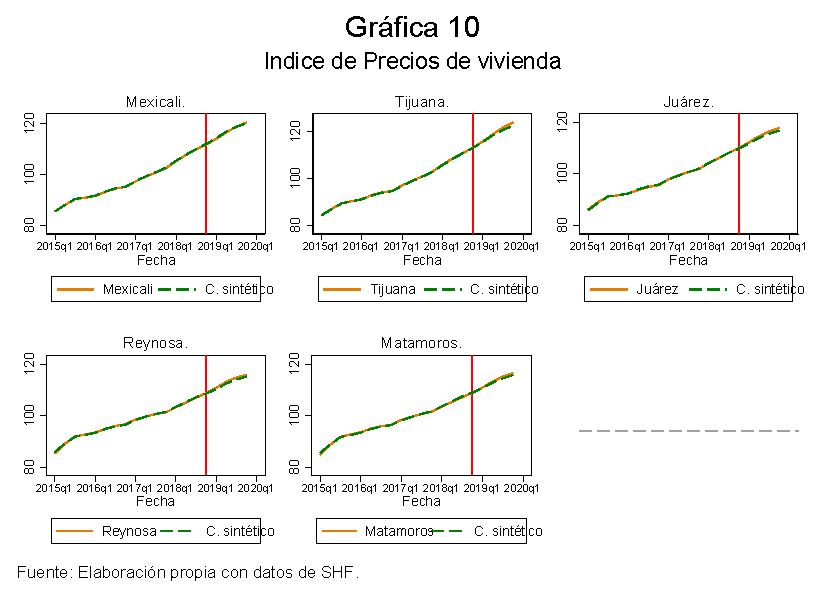
\includegraphics[width=\textwidth]{Figures/synth.pdf}
\caption{Control sintético para precios de vivienda.}
\label{fig:10}
\end{figure}


	% \chapter{Discusión}
\label{ch:conclusions}

%\begin{chapterquote}{Leslie Lamport}
%	Formal mathematics is nature's way of letting you know how sloppy
%your mathematics is.
%\end{chapterquote}

%Yo empezaría por resumir lo que hiciste:
%Este trabajo responde a la pregunta del impacto de X en Y. Siguiendo el método Z, encontré W. 
%Después diría posibles interpretaciones o implicaciones de política pública. ¿Por qué tiene valor lo que hiciste?
%Por último, recalcaría limitaciones de tu análisis: datos y metodología.

\noindent Este trabajo presenta una primera aproximación al impacto del aumento del salario mínimo en el mercado inmobiliario, en particular al acceso a vivienda para quienes perciben menores ingresos. A partir del método de diferencias en diferencias logro aislar el efecto promedio de subir el salario mínimo en el empleo y salario para trabajadores registrados ante el IMSS, el efecto en los créditos INFONAVIT, en las hipotecas privadas y en los precios de vivienda. 

Encuentro que aumentar el salario mínimo no afectó ni al empleo, ni a los créditos privados ni a los precios de vivienda. Sin embargo, sí causó que aumentaran tanto el salario reportado ante el IMSS (en mayor medida para quienes menor salario tienen) como el crédito INFONAVIT. Cabe resaltar que no puedo hablar de un aumento en el ingreso laboral, ya que no tengo evidencia de que el aumento al salario no se dio a costa de una reducción en prestaciones.

La principal implicación de política pública de mi análisis es que conduce a pensar que las medidas encaminadas a aumentar el porcentaje del salario que es reportado por los patrones trae mejoras al bienestar de quienes menos ganan. Al cotizar con mayores salarios ante el IMSS pueden obtener más crédito INFONAVIT y enfrentar en promedio los mismos precios de vivienda. Entonces, pueden adquirir mejores hogares, posiblemente más cerca de los centros de trabajo o con mejores servicios.



Todos los datos que utilicé son de acceso público, disponibles en las bases de datos de las distintas instituciones (IMSS,INFONAVIT,SHF,CNBV) que cito. En ese sentido, mis conclusiones están limitadas por los datos que están disponibles al público. Para llegar a mejores conclusiones sería necesario contar con datos más desagregados. En concreto, dado que cada sector de la distribución de salario demanda distintas opciones de vivienda, un análisis de heterogeneidad sería altamente valioso. 

Como los datos para el precio proviene de un índice agregado, este análisis carece de herramientas para determinar si quizás se suscitaron  movimientos en los precios de las casas demandadas por quienes ganan menos. Se podría dilucidar este cuestionamiento   si los microdatos que se utilizaron para construir el índice fuesen de acceso público.

Quizá mis conclusiones serían más profundas si pudiera analizar por banco, ya que hay bancos que atienden a un sector particular de la demanda. Sería interesante ver un análisis en crédito al consumo, donde puede ser que las viviendas recién adquiridas se utilicen como colateral para financiar otro tipo de inversiones.

Más importante aún, puede ser que el efecto de aumentar el salario mínimo se diluya por otros canales que no observamos. Por ejemplo, quienes ganan menos salarios regularmente rentan en lugar de comprar. Además, quienes compran adquieren viviendas con características distintas a quienes se ubican en otros puntos de la distribución de salarios. Entonces, mi análisis se encuentra limitado al no tener datos sobre las rentas de vivienda.

Finalmente, es imposible distinguir si un movimiento en precios agregados por aumentar el salario mínimo proviene del puro efecto ingreso o del canal de crédito. En caso de disponer de microdatos, podría seguir un análisis como el propuesto por \citep{diamond_2016} para capturar qué tanto valoran los individuos vivir en una región con un salario mínimo comparativamente más alto.


	%%%%%%%%%%%%%%%%%%%%%%%%%%%%%%%%%%%%%%%%%%%%%%
	% APPENDIX
	%%%%%%%%%%%%%%%%%%%%%%%%%%%%%%%%%%%%%%%%%%%%%%
	\appendix
	% \include{Chapters/appendixA}

	%%%%%%%%%%%%%%%%%%%%%%%%%%%%%%%%%%%%%%%%%%%%%%
	% BIBLIOGRAPHY
	%%%%%%%%%%%%%%%%%%%%%%%%%%%%%%%%%%%%%%%%%%%%%%
	\clearpage
	\addcontentsline{toc}{chapter}{References} %Añadimos la bibliografia a la lista de contenidos.
	
	%%%%%%%%% Referencias usando el sistema embedido %%%%%%%%%%%
	% e.g. (Ejemplo tomado de https://en.wikibooks.org/wiki/LaTeX/Bibliography_Management)
	%
	% \begin{thebibliography}{9}
	%
	%	\bibitem{lamport94}
    %			Leslie Lamport,
    %			\emph{LaTeX: a document preparation system},
    %			Addison Wesley, Massachusetts,
  	%			2nd edition,
    % 			1994.
    %
	% \end{thebibliography}

	%%%%%%%%% Referencias usando bibtex %%%%%%%%%%%
	\bibliographystyle{plain}
	\bibliography{references} 

\end{document}